\section{Published mechanisms in the earlier simulator}\label{sec:mech}

\begin{figure*}[t]
\centering
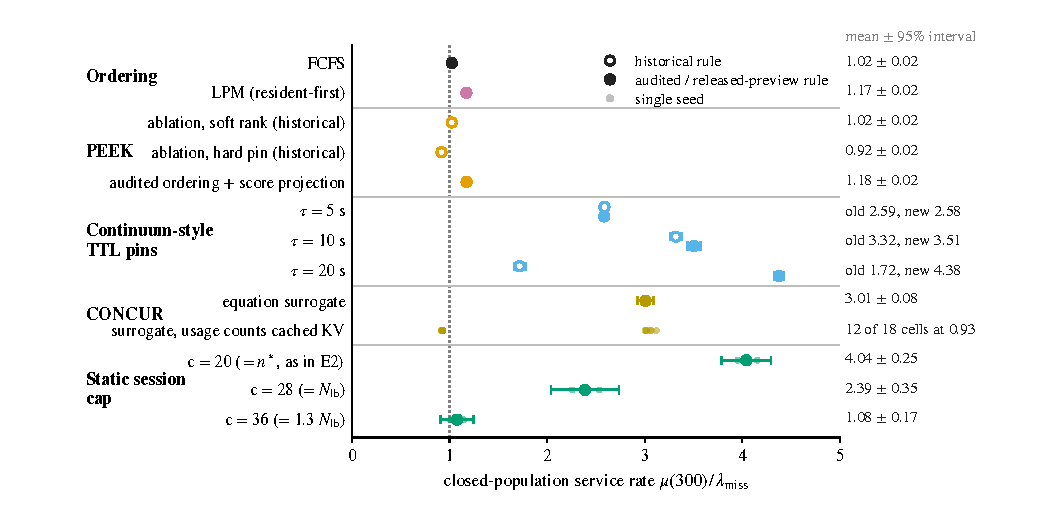
\includegraphics[width=0.92\textwidth]{figs/fig4_mechanisms.pdf}
\caption{$\mu(300)/\lmiss$, our proxy for the congested service rate $\muinf$, per mechanism in the earlier, uncalibrated simulator: mean over 10 seeds with 95\% $t$ intervals, in units of that simulator's $\lmiss$ (0.0474\sps; not comparable with Figs.~\ref{fig:curve}--\ref{fig:edge}); the intervals omit the 1.5\% standard error of $\lmiss$. Hollow: ablations (PEEK's queued-prefix protection under FCFS order, as a soft rank and as a hard-pin counterfactual PEEK does not apply; fixed pins held until expiry even with the GPU idle). Filled: all other rows; for PEEK, a projection of its released scheduler; for the pins, fixed TTLs under the preview's release rule (values: held until expiry, preview). LPM is pure LPM, without SGLang's 128-request fallback. CONCUR: a surrogate of its control equation; small dots: 18 cells in which finished sessions' KV counts as usage. Static caps $c=20$ (E2's cap; this simulator's $n^*$ is 22), 28, 36: $\mu(c)$ of the closed FCFS curve (3 other seeds, not paired with the other rows).}\label{fig:mech}
\end{figure*}

In the fluid model of \S\ref{sec:fluid} the recovery threshold from deep congestion is at most $\muinf$, so a mechanism can raise it only as far as it raises $\muinf$. We compare mechanisms by $\mu(300)/\lmiss$ as a proxy for $\muinf$ (Fig.~\ref{fig:mech}) in the earlier, uncalibrated simulator. Each rule was compared, by reading the code and not running it, with the released code where it exists (PEEK; the Continuum preview, which omits the paper's estimator) or with the paper (CONCUR, for which we found no code); where a difference was small and unambiguous we added a projection of the released rule beside the historical row, and the differences that remain are stated below. That simulator's assumed costs are about 1.5 times the fitted ones ($\lmiss$ 0.0474 against 0.0722\sps), and its curve peaks at 4.07 times its own $\lmiss$, against about 3.0 in the calibrated simulator and $3.26\,\lref$ on the engine. Its absolute rates therefore do not carry over. As in Stage~C, all sessions start at $t=0$, but each run is measured over 25,000\,s after a 5000\,s warmup (static caps: 30,000\,s), about four mean session lifetimes; FCFS reads 1.04 $\lmiss$ over the first half of the window and 1.01 over the second, so the synchronized-start bias of \S\ref{sec:diag} is a few percent here. These are results about the rules in a workload with private prefixes and exponential 5\,s tools, not benchmarks of the named systems.

\paragraph{Orderings.} FCFS gives $1.024\pm0.020$ with hit fraction 0.000 and the GPU always busy; with the 1.5\% standard error of $\lmiss$ included the interval is $1.02\pm0.04$, consistent with Proposition~\ref{prop:A}, which covers this simulator's request-level FCFS. Pure LPM (without SGLang's 128-request fallback) gives $1.174\pm0.023$ and recovers from 300 cold sessions over 150,000\,s up to 1.1 $\lmiss$, not at 1.25. PEEK~\citep{xie2026peek} protects prefixes needed by queued requests and adds a cache-aware scheduler. Our earlier rows implemented only the protection under FCFS order. As a soft ranking, which is how PEEK's eviction hook protects (finite priorities), it gives the same throughput as FCFS seed for seed: queued requests' KV is protected but still evicted before FCFS admits them (2,831--3,128 such evictions per run), so no request is admitted with its KV, consistent with Proposition~\ref{prop:A}. A hard pin, a counterfactual PEEK does not apply, gives 0.919. The released scheduler serves warm requests first; projected onto single-session prefixes with its eviction score, it gives $1.176\pm0.021$, equal to pure LPM within $0.001\pm0.014$, and recovers from none of 5 bursts at 2 $\lmiss$. Here PEEK is an LPM-class ordering, not FCFS; we did not evaluate it on shared-prefix traffic, for which it is designed.

\paragraph{TTL pins.} Continuum keeps a program's KV after a non-final turn for a time-to-live chosen by a cost model, which may be zero~\citep{li2025continuum}. Its released preview omits that estimator: it pins for 2\,s, and only when the parsed tool's historical mean is at most 2\,s, so it would rarely pin our 5\,s-mean tool calls. We did not implement the paper's estimator. Our rows are therefore fixed, unconditional TTLs of $\tau=5$, 10 and 20\,s on every non-final turn, with Continuum's waiting order (pinned programs first). Under the preview's release rule (when an allocation fails and nothing runs, release the pin that expires last) they give $2.584\pm0.035$, $3.505\pm0.064$ and $4.376\pm0.048$; at $\tau=20$\,s the system recovers from a cold start up to 4.0 $\lmiss$ and from 5 of 5 bursts. Under the rule we read in the paper's deadlock-prevention text (when a request does not fit, unpin the latest-arriving programs until it fits, also while work runs), $\tau=10$ and 20\,s give 1.16--1.17 and recover from no cold start at 1.1 $\lmiss$ or above and from no burst. Our earlier rule, which waited for expiry while the GPU idled, gave 1.719 at $\tau=20$\,s. With plain FCFS order instead of Continuum's, under that earlier rule, the pins gave 0.29, 0.17 and 0.10 at $\tau=5$, 10 and 20\,s (3 seeds), with the GPU busy 33\%, 17\% and 8\% of the time: that simulator keeps an expired pin while the session's next request waits, which under FCFS lasts the rest of the queue wait. This is consistent with Proposition~\ref{prop:A}. These are results about configured pins, not about Continuum.

\paragraph{Adaptive caps.} CONCUR adds 2 to a window on active agents when KV usage is below 0.2 and halves it when usage exceeds 0.5 and the hit rate is below 0.2~\citep{chen2026concur}; we found no released code. Our session-gate surrogate of this equation gives $3.009\pm0.081$ and recovers from 5 of 5 bursts. It depends on the usage signal: if finished sessions' KV, still cached and evictable, counts as usage, 12 of 18 cells stall at our surrogate's minimum window of 4 at 0.915--0.935 $\lmiss$; of five exploratory sensitivities, one (a 5\,s control interval instead of our surrogate's 10\,s) raised the rate by $0.184\pm0.167$, an unadjusted pointwise interval. Pause and resume of admitted agents is not modelled. So 3.0 is the surrogate's rate under a live-sessions-only usage signal, not deployed CONCUR's threshold.

\paragraph{Static caps.} By Proposition~\ref{prop:cap} a cap $c$ holds a large population at $\mu(c)$: $4.04\pm0.25$ at $c=20$, $2.39\pm0.35$ at $c=28\approx\Nlb$ and $1.08\pm0.17$ at $c=36$ (3 seeds), against a peak of 4.07 at $n=22$. The cliff makes the choice fragile: a cap about a quarter above $\Nlb$ is back near $\lmiss$.

\paragraph{Admission by memory demand.} ThunderAgent periodically compares the programs' KV demand with the capacity, counting a program in a tool call at a weight that decays with its tool time ($2^{-t}$ in its experiments). When demand exceeds capacity it pauses whole programs, those in tool calls and those with the shortest contexts first, and it restores them when demand falls; both watermarks are set to 1 in its evaluation~\citep{kang2026thunderagent}. NVIDIA Dynamo ships a port that pauses programs at tool boundaries, by default when utilization reaches 0.95 of the pool, down to 0.80, and resumes them at 0.85 or below~\citep{dhanani2026dynamo}. This is an implemented form of a session bound, sized by memory demand rather than count; we have not evaluated it. Proposition~\ref{prop:cap} concerns a FIFO count cap whose sessions keep their slots, so it does not predict a gate that bounds current demand and pauses admitted programs. The static-cap rates above are not a prediction for either system.

\paragraph{Why the ranking comes out this way.} Under request-level FCFS, with or without protection that keeps FCFS order, $\muinf$ cannot exceed $\lmiss$ when (A3) holds (Proposition~\ref{prop:A}); we conjecture (Remark in \S\ref{sec:props}) that pure resident-first orderings raise it through tool calls shorter than the congested lifetime of idle KV, and for pure LPM the simulator agrees. A static cap $c$ holds the engine at $\mu(c)$ (Proposition~\ref{prop:cap}), so at most at the peak, 4.07 at $n=22$ (3 seeds). Pins at $\tau=20$\,s gave 4.38, above every static cap we ran and above the peak, though within the peak's 3-seed interval ($\pm0.36$). In this simulator they also serve pinned programs first and keep a returning session's KV for at least $\tau$, and the set of sessions they bound depends on memory, not on a count; we have not separated these effects. On the real engine, stock LPM recovered from a 200-session burst at 1.35 $\lref$ in 4 of 6 runs (\S\ref{sec:grid}); that finite-burst result does not compare directly with these deep-congestion rates, and in deep congestion stock LPM stops re-sorting its queue, so, on our reading of its source, Proposition~\ref{prop:A} bounds its $\muinf$ by $\lmiss$ when (A3) holds.
